% !TeX root = progress2.tex

\subsubsection{Progress}

This is a quick summary of tasks I have done:
\begin{description}
    \item[$\bullet$] Worked on further structuring simulation code, allowing to test any defined alphabet and common methods and functions for autoencoder, data processing and graph making.
	\item[$\bullet$] Pre-trained autoencoder's encoder and decoder separately with a known 16QAM alphabet and let it train further as single model. Reason for this was to start model with know local minimum and hopefully find slightly better result to given alphabet (as autoencoder usually finds local minimum that produces alphabet that is not in gray-coding). This test failed, however it allowed improving encoder and decoder models. 
	\item[$\bullet$] Tested autoencoder's performance when trained with different noise levels.
	\item[$\bullet$] Started to implement HDL code with some skeleton structure.
	\item[$\bullet$] Implemented a standalone code for a trained neural network. This was a simple test to see how difficult it is to extract weights and biases from trained tensorflow model and replicated structure with pure python code (without libraries). This leads to next step of implementing it in HDL. 
	\item[$\bullet$] Tested new tensorflow feature of post-training quantisation - it converts native tensorflow 32bit floating point values (F32) to lower precision values. I16x8 shows the worst performance however it is most promising to implement on an FPGA due to lack of floating point computation.

    \begin{figure}[H]
        \centering
        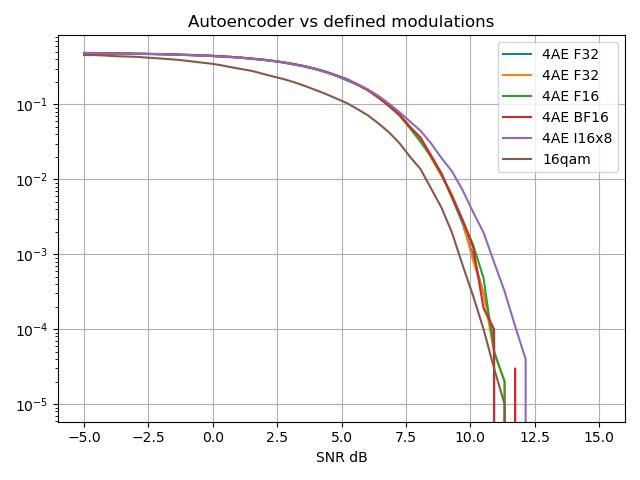
\includegraphics[width=.75\linewidth]{post-train-quan.jpg}
        \caption{BER/SNR graph with 4bit AutoEncoder (4AE) with different post-training quantisaion - 32bit and 16bit floating point (F32 and F16); 16bit Brain Floating Point (BF16) \autocite{bfloat16}; 16bit integer for activation and 8bit integer for weights (I16x8) \autocite{i16x8}}
    \end{figure}
    
    \item[$\bullet$] Helped researching available and suitable FPGAs, ADCs and DACs. 


\end{description}


\subsubsection{Difficulties Encountered}
\begin{description}
    \item[$\bullet$] Difficulties with time management and stress due to other module deadlines
    \item[$\bullet$] Overwhelming amount of information with FPGAs, ADCs and DACs.
\end{description}